\chapter{Photogrammetrie}

\section{Einführung in die Photogrammetrie}

Das Grundprinzip der Messung mit Kameras ist einfach. Licht breitet sich mit einer bestimmten Wellenlänge, in annähernd geraden Strahlen aus. Diese Strahlen werden vom Sensor der Kamera aufgenommen, sodass diese die Richtungen im dreidimensionalen Raum misst. Der grundlegende geometrische Zusammenhang der Photogrammetrie ist somit die Zentralprojektion, die sich mathematisch durch die Kollinearitätsgleichung beschreiben lässt. Ein dreidimensionaler Punkt in der echten Welt, sein Bild in der Kamera und das Projektionszentrum müssen alle auf einer geraden Linie liegen. (vgl. \cite{fiundations_pg} S.1) Das fundamentale photogrammetrische Problem besteht in der Bestimmung von internen und externen Ausrichtungsparametern der Kamera und der  Messung von Objekt und Raumkoordinaten der aufgenommenen Fotografien. 


\begin{itemize}
\item \textbf{Interne Orientierung}: Bei der internen Orientierung werden Kameraparameter gemessen und ausgewertet. Dazu wird die \glqq principle distance\grqq{} (Brennweite) und der \glqq principle point\grqq{} (Optisches Zentrum) betrachtet.

\begin{figure}[H]
	\centering
	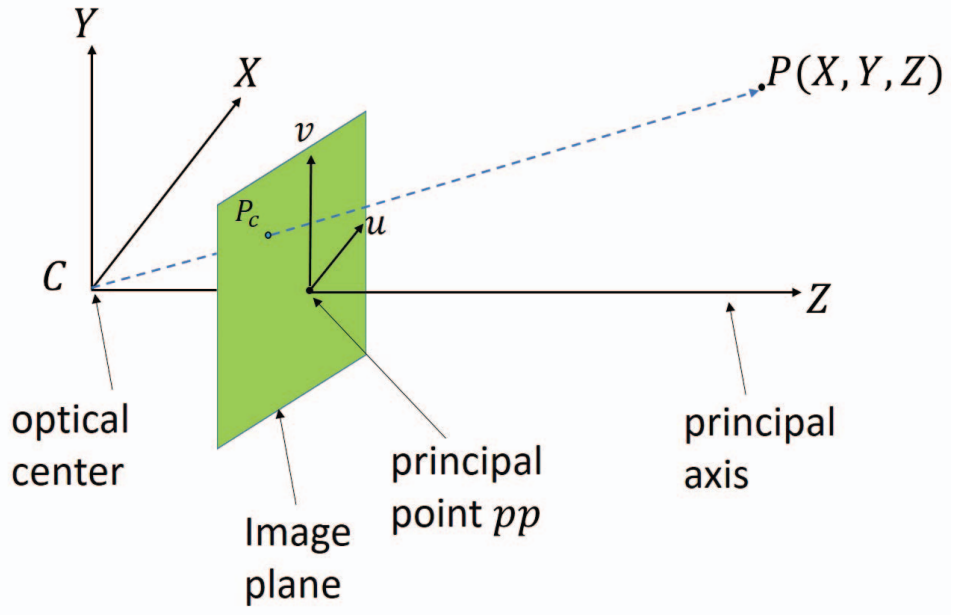
\includegraphics[scale=0.45]{pp.png}
	\caption{Kamera Kalibierungsmodell, Bildquelle \cite{pp}}
\end{figure} 

Weiterhin müssen Parameter, welche die Verzeichnung, also die nicht maßstabsgetreue Abbildung von Objekten, betrachtet werden. Diese Parameter, die beispielsweise in der Objektivkorrektur verwendet werden, müssen, um die interne Orientierung der Kamera genau abzubilden, mit in die Berechnung einfließen.

\item \textbf{Externe Orientierung}: Bei der externen Orientierung wird versucht die genaue räumliche dreidimensionale Lage der Kamera zum Zeitpunkt der Belichtung des Bildes zu rekonstruieren. Für die Bestimmung der Orientierung von ein oder mehreren Fotos, können verschiedene Methoden verwendet werden. Dies kann in Teilschritten (relative und absolute Orientierung) oder gleichzeitig (Bündelblockausgleich) durchgeführt werden. (vgl. \cite{exterior_review} S.616)
\end{itemize}

Khalid El-AShmawy \cite{comparative_conditions_study} beschreibt die Verwendung von Strahlenbündel, die durch Fotos generiert werden, als zweifelsfrei den flexibelsten Ansatz zur Blockbildung, Blockanpassung und für Photogrammetrie im Allgemeinen und mit den besten Ergebnissen. In der Nahbereichsphotogrammetrie, bei der mehrstufige und konvergente Konfigurationen möglich sind, ist der Bündelansatz in seiner stärksten Form vertreten. 


Der Ausgleich der Strahlenbündel in einem Set an Fotos beinhaltet die Rotation und Translation von jedem Bündel im Raum in eine Position, in der alle Strahlen sich an der korrekten Position im Objektraum schneiden. (vgl. \cite{comparative_conditions_study} S.66)

\section{Bündelblockausgleich}

Das Verfahren des Bündelblockausgeleichs, verwendet die Methoden der \glqq collinearity condition \grqq{} (Kollinearitätsbedingung), der \glqq coplanarity condition\grqq{} (Koplanaritätsbedingung) oder die Methode der direkten linearen Transformation. Die gewünschten Parameter aller Fotos werden gleichzeitig durch eine iterative Wiederholung der \glqq least square\grqq{} Methode (Methode der kleinsten Quadrate) angepasst und korrigiert. Die Iterationen sind durch die nicht-Linearität der Konditionsgleichungen notwendig. Die Resulate des Bündelblockausgleichs aller Fotos sind dann die Ergebnisse der externen Orientierung der Kamera für jedes einzelne Foto. Weiterhin ergibt sich eine Auflistung der Objektraumkoordinaten der gemessenen Punkte aller Fotos, sowie deren gemessene statische Genauigkeit. (vgl. \cite{comparative_conditions_study} S.66-67)

\url{https://ethz.ch/content/dam/ethz/special-interest/baug/igp/photogrammetry-remote-sensing-dam/documents/pdf/math-of-photogrammetry.pdf}
\url{http://sci-hub.tw/https://doi.org/10.3846/20296991.2015.1051335}
\url{http://sci-hub.tw/10.1111/0031-868X.00210}

\subsection{Bestimmung der externen Kameraparameter mit der Kollinearitätsbedingung}

Die gleichzeitige Anpassung verwendet die Kollinearitätsbedingung  um zwei Gleichungen für jeden gemessenen Bildpunkt aufzustellen. Die Lösung all dieser Gleichungen erfolgt dann nach der Methode der kleinesten Quadrate. Die Bedingung der Kollinearität sagt aus, dass ein Objektpunkt $P$, sein Bildpunkt $p$ und das perspektivische Zentrum $O$, alle auf der gleichen Geraden liegen müssen. Mathematisch wird die Bedingung wie folgt ausgedrückt  \cite{coll_exterior}:

\begin{equation}
\begin{aligned}
  x_p = -f \frac{(X_p-X_O)m_{11}+(Y_p-Y_O)m_{12}+(Z_p-Z_O)m_{13}}{(X_p-X_O)m_{31}+(Y_p-Y_O)m_{32}+(Z_p-Z_O)m_{33}} \\
    y_p = -f \frac{(X_p-X_O)m_{21}+(Y_p-Y_O)m_{22}+(Z_p-Z_O)m_{23}}{(X_p-X_O)m_{31}+(Y_p-Y_O)m_{32}+(Z_p-Z_O)m_{33}}
\end{aligned}
\end{equation}

Dabei sind $x_p$ und $y_p$ die korrigierten Foto Koordinaten, $X_p,Y_p,Z_p$ die Objektpunktkoordinaten von $P$, $X_O,Y_O,Z_O$ die Koordinaten des perspektivischen Zentrums $O$, $f$ die kalibrierte Brennweite der Kamera und $m_{ij}$ die Elemente der Orientierungsmatrix $M$ des Fotos.

Die linearisierte Form der Gleichung, für die Lösung der Methode der kleinsten Quadrate, wird gegeben als (\cite{comparative_conditions_study} S.67):

\begin{equation}
V+B\cdot\triangle =\varepsilon
\end{equation}

Wobei:
\begin{itemize}
\item $\triangle$ der Korrekturvektor zu dem aktuellen Werteset, für die unbekannten Werte (innere und äußere Orientierung, Objektkoordinaten der Punkte) der iterativen Lösung ist.

\item $B$ die Matrix der partiellen Ableitungen von Gleichung (3.1), in Bezug auf die Unbekannten  ist.

\item $V$ der Korrekturvektor zu den Beobachtungen ist.

\item $\varepsilon$ der Abweichungsvektor ist.
\end{itemize}

El-Ashmawy \cite{comparative_conditions_study} schlägt weitere Beschränkungen vor, indem ergänzende Beobachtungsgleichungen berücksichtigt werden, die sich aus den a priori Kenntnissen der Raumkoordinaten der Objekte der Kontrollpunkte in Gleichung (3.2) ergeben. Solche zusätzlichen Gleichungen können wie folgt beschrieben werden:

\begin{equation}
V^c-\triangle^c = \varepsilon^c
\end{equation}

Wobei:

\begin{itemize}
\item $\triangle^c$ der Vektor der beobachtbaren Korrekturen zu den Objektkoordinaten der Kontrollpunkte ist.

\item $\varepsilon^c$ der Abweichungsvektor zwischen Beobachtungswerten und aktuellen (in iterativer Lösung) Werten der Objektkoordinaten der Kontrollpunkte ist.

\end{itemize}

Beobachtungsgleichungen können dann durch das Zusammenführen von Gleichung (3.2) und (3.3) erhalten werden. Die grundlegenden Voraussetzungen an den Bündelblockausgleich sind die Schätzungen der Parameter für innere und äußere Orientierung der Kamera. Weiterhin können die - je nach spezifischem Ansatz - Schätzungen für die Objekt und Raumkoordinaten aller Kontrollpunkte  nützlich sein. Deshalb sollte ein Bündelverfahren immer eine praktikable Methode enthalten, mit der die ungefähren geschätzten initialen Werte ermittelt werden können. Dieses Vorwissen sorgt nicht nur für eine reduzierte Anzahl an Iterationen, sondern resultiert auch in schnelleren und genaueren Ergebnissen. (vgl. \cite{comparative_conditions_study} S.67)


\subsection{Bestimmung der externen Kameraparameter mit der Koplanaritätsbedingung}

Die Koplanaritätsbedingung impliziert, dass die beiden perspektivischen Zentren von zwei Aufnahmen, ein beliebiger Objektpunkt und die entsprechenden Bildpunkte auf den beiden Fotos, alle in einer gemeinsamen Ebene liegen müssen (vgl. Abbildung 3.2). Die Koplanaritätsbedingung kann wie folgt dargestellt werden (\cite{pose_est_epi} S.1204):

\begin{equation}
F_i = \begin{vmatrix}
b_X & b_Y & b_Z \\
X_1 & Y_1 & Z_1 \\
X_2 & Y_2 & Z_2
\end{vmatrix}
=0
\end{equation}

Dabei sind $b_X,b_Y,b_Z$ die Komponenten des Basisvektors $b$ und $X_1,Y_1,Z_1$ sowie $X_2,Y_2,Z_2$ sind die Komponenten des Vektors $\vec{R_1}$ (von $O_1$ zu $P$) respektive  $\vec{R_2}$ (von $O_2$ zu $P$).


\begin{figure}[H]
	\centering
	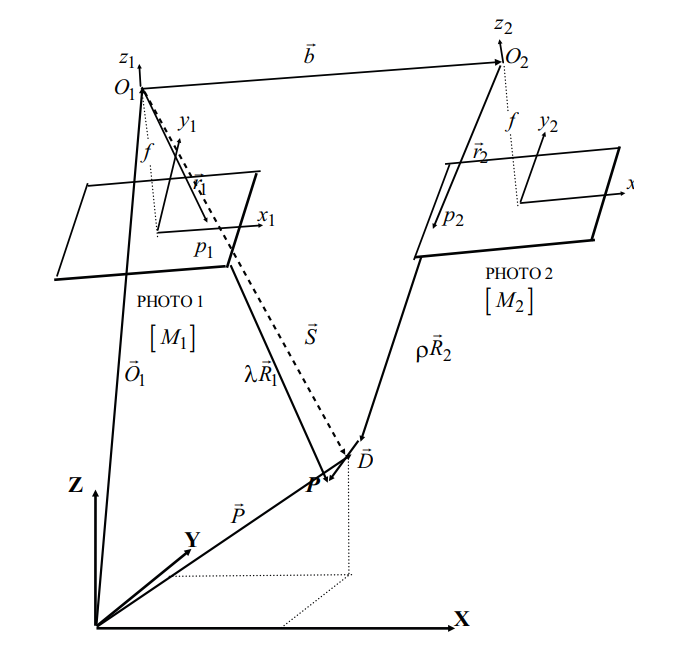
\includegraphics[scale=0.6]{coplanarity.png}
	\caption{Koplanaritätsbedinung, Bildquelle \cite{comparative_conditions_study}}
\end{figure} 

Das mathematische Modell besteht aus vier skalaren Gleichungen:

\begin{equation}
\begin{aligned}
X_p - (X_{O_1}+0.5(b_X+ \lambda \cdot X_1 + p \cdot X_2)) = 0.0 \\
Y_p - (Y_{O_1}+0.5(b_Y+ \lambda \cdot Y_1 + p \cdot Y_2)) = 0.0 \\
Z_p - (Z_{O_1}+0.5(b_Z+ \lambda \cdot Z_1 + p \cdot Z_2)) = 0.0 \\
D_Y = \lambda\cdot X_1-p\cdot X_2-b_Y = 0.0
\end{aligned}
\end{equation}

Wobei $X_{O_1}, Y_{O_1},Z_{O_1}$ die Objektkoordinaten der ersten Kameraposition während der Belichtung sind und $\lambda$ und $p$ die Skalierungsfaktoren der entsprechenden Positionsvektoren $\vec{r_1}$ und $\vec{r_2}$ im Kameraraum sind. 

Die linearisierte Form von Gleichung (3.5), mit ebenfalls von El-Ashmawy \cite{comparative_conditions_study} vorgeschlagenen zusätzlichen Beschränkungen, für das Verfahren der kleinsten Quadrate, wird gegeben als:

\begin{equation}
\begin{aligned}
A\cdot V + B\cdot \triangle = \varepsilon \\
V^c - \triangle^c = \varepsilon^c
\end{aligned}
\end{equation}


Wobei:
\begin{itemize}
\item $\triangle$ der Korrekturvektor zu dem aktuellen Werteset, für die unbekannten Werte (innere und äußere Orientierung, Objektkoordinaten der Punkte) der iterativen Lösung ist.

\item $A$ die Matrix der partiellen Ableitungen von Gleichung (3.5), in Bezug auf die Beobachtungen (korrigierte Foto-Koordinaten auf den linken und rechten Fotos, des gleichen Objektpunkts) ist.

\item $B$ die Matrix der partiellen Ableitungen von Gleichung (3.5), in Bezug auf die Unbekannten  ist.

\item $V$ der Korrekturvektor zu den Beobachtungen ist.

\item $\varepsilon$ der Abweichungsvektor ist.
\end{itemize}

Zur Verwendung der iterativen Lösung der kleinsten Quadrate, ist die Berechnung der Ausgangswerte von Unbekannten, wie beim Verfahren mit der Kollinearitätsbedinung, notwendig.


\subsection{direct linear transformation}

\subsection{Feature Matching}

\subsection{Image Matching}

\subsection{Structure from Motion}

6.2 Structure from motion

\url{http://sci-hub.tw/https://doi.org/10.1007/s10462-012-9365-8}

\subsection{Depth Maps}

\section{Photogrammetrie für Smartphones}

\section{Evaluierung der photogrammetrischen Technologie für Echtzeit AR Anwendungen}